\subsection{Hough transform}
\label{sec:locate:hough}

The Hough transform~\cite{hough} is a technique commonly used in computer vision to find specific patterns, such as lines of circles.
Here, a circular Hough transform is used to identify bubbles, which have a mostly circular shape.
The implementation used is the function \texttt{HoughCircles} provided by \texttt{OpenCV}.

\subsubsection{Algorithm}

The Hough transform operates the following algorithm:
\begin{enumerate}
	\itemsep 0em
	\item Use the Canny filter to identify the edges within the image;
	\item For each pixel of this resulting image:
	      \begin{enumerate}
		      \item For growing radii $r$, compute the percentage $p_r$ of the pixels that are ``on'' within the ones at distance $r$ from the considered pixel;
		      \item Take note of $P = max(p_r)$ and $R = argmax(p_r)$ for the pixel;
		      \item Filter out pixels whose $P$ is lower than a chosen threshold (no meaningful circle is found around them);
	      \end{enumerate}
	\item Perform non-max suppression on the values of $P$ of all pixels;
	\item Consider all the remaining pixels as bubbles, of corresponding radius $R$.
\end{enumerate}

\subsubsection{Evaluation}

Figure~\ref{fig:locate:hough} shows the results of the algorithm: about 84\% of the bubbles were found, at a speed of 55 FPS.

\begin{figure}
	\centerline{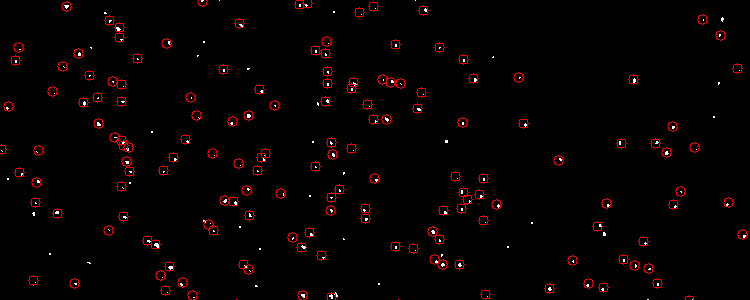
\includegraphics[width=\locateimgsize]{images/locate/hough-transform.png}}
	\caption{\centering Hough's result}
	\label{fig:locate:hough}
\end{figure}
